\section{Aufbau}
\label{sec:Aufbau}

Der Versuchsaufbau besteht aus einem Ultraschallechoskop, zwei Ultraschallsonden die mit $\SI{2}{\mega\hertz}$ betrieben werden und einem Computer zu Aufnahme und Analyse der Messdaten. Als Proben dienen verschieden lange Acrylzylinder und verschieden dicke Acrylplatten. Als Kopplungsmittel dienen destilliertes Wasser und Koppelgel. Am Ultraschallechoskop kann die Messmethode auf Durchschallungs- oder Impuls-Echo-Verfahren gestellt werden. Zur Auswertung der Messdaten am Computer wird die Software A-Scan verwendet. Für den letzten Versuchsteil wird ein Augenmodell wie in Abbildung \ref{fig:Augenmodell} verwendet. 
\begin{figure}
\centering
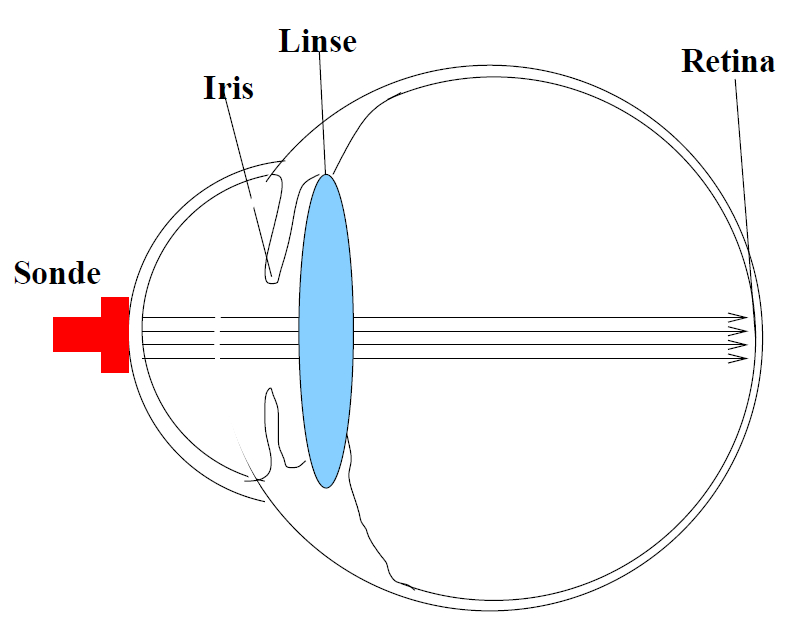
\includegraphics[scale=0.3]{content/images/Augenmodell.jpg}
\caption{Schematischer Aufbau des Augenmodells \cite{US1}}
\label{fig:Augenmodell}
\end{figure}